\chapter*{Funkcjonalność projektu}
Projekt jest wysoce wyspecjalizowany -- aplikacja przeprowadza wyłącznie proces symulacji i uczenia. Użytkownik może konfigurować ustawienia tego procesu.
\section*{Wymagania funkcjonalne}
\begin{itemize}
	\item Przeprowadzenie procesu uczenia optymalnych czasów świecenia sygnalizatorów na skrzyżowaniu za pośrednictwem algorytmu ewolucyjnego,
	\item Konfiguracja ustawień symulacji, będącej bazą procesu uczenia,
	\item Konfiguracja ustawień algorytmu ewolucyjnego,
	\item Wyświetlanie na bieżąco informacji o przebiegu uczenia ,
	\item Wyświetlenie wyników uczenia po jego zakończeniu.
\end{itemize}
\section*{Wymagania pozafunkcjonalne}
\begin{itemize}
	\item Stabilność -- aplikacja musi pracować bezawaryjnie przez wiele godzin,
	\item Wydajność -- aplikacja musi działać na tyle wydajnie, aby symulacja mogła być przeprowadzana kilkadziesiąt razy szybciej niż czas rzeczywisty.
\end{itemize}
\begin{figure}
	\centering
	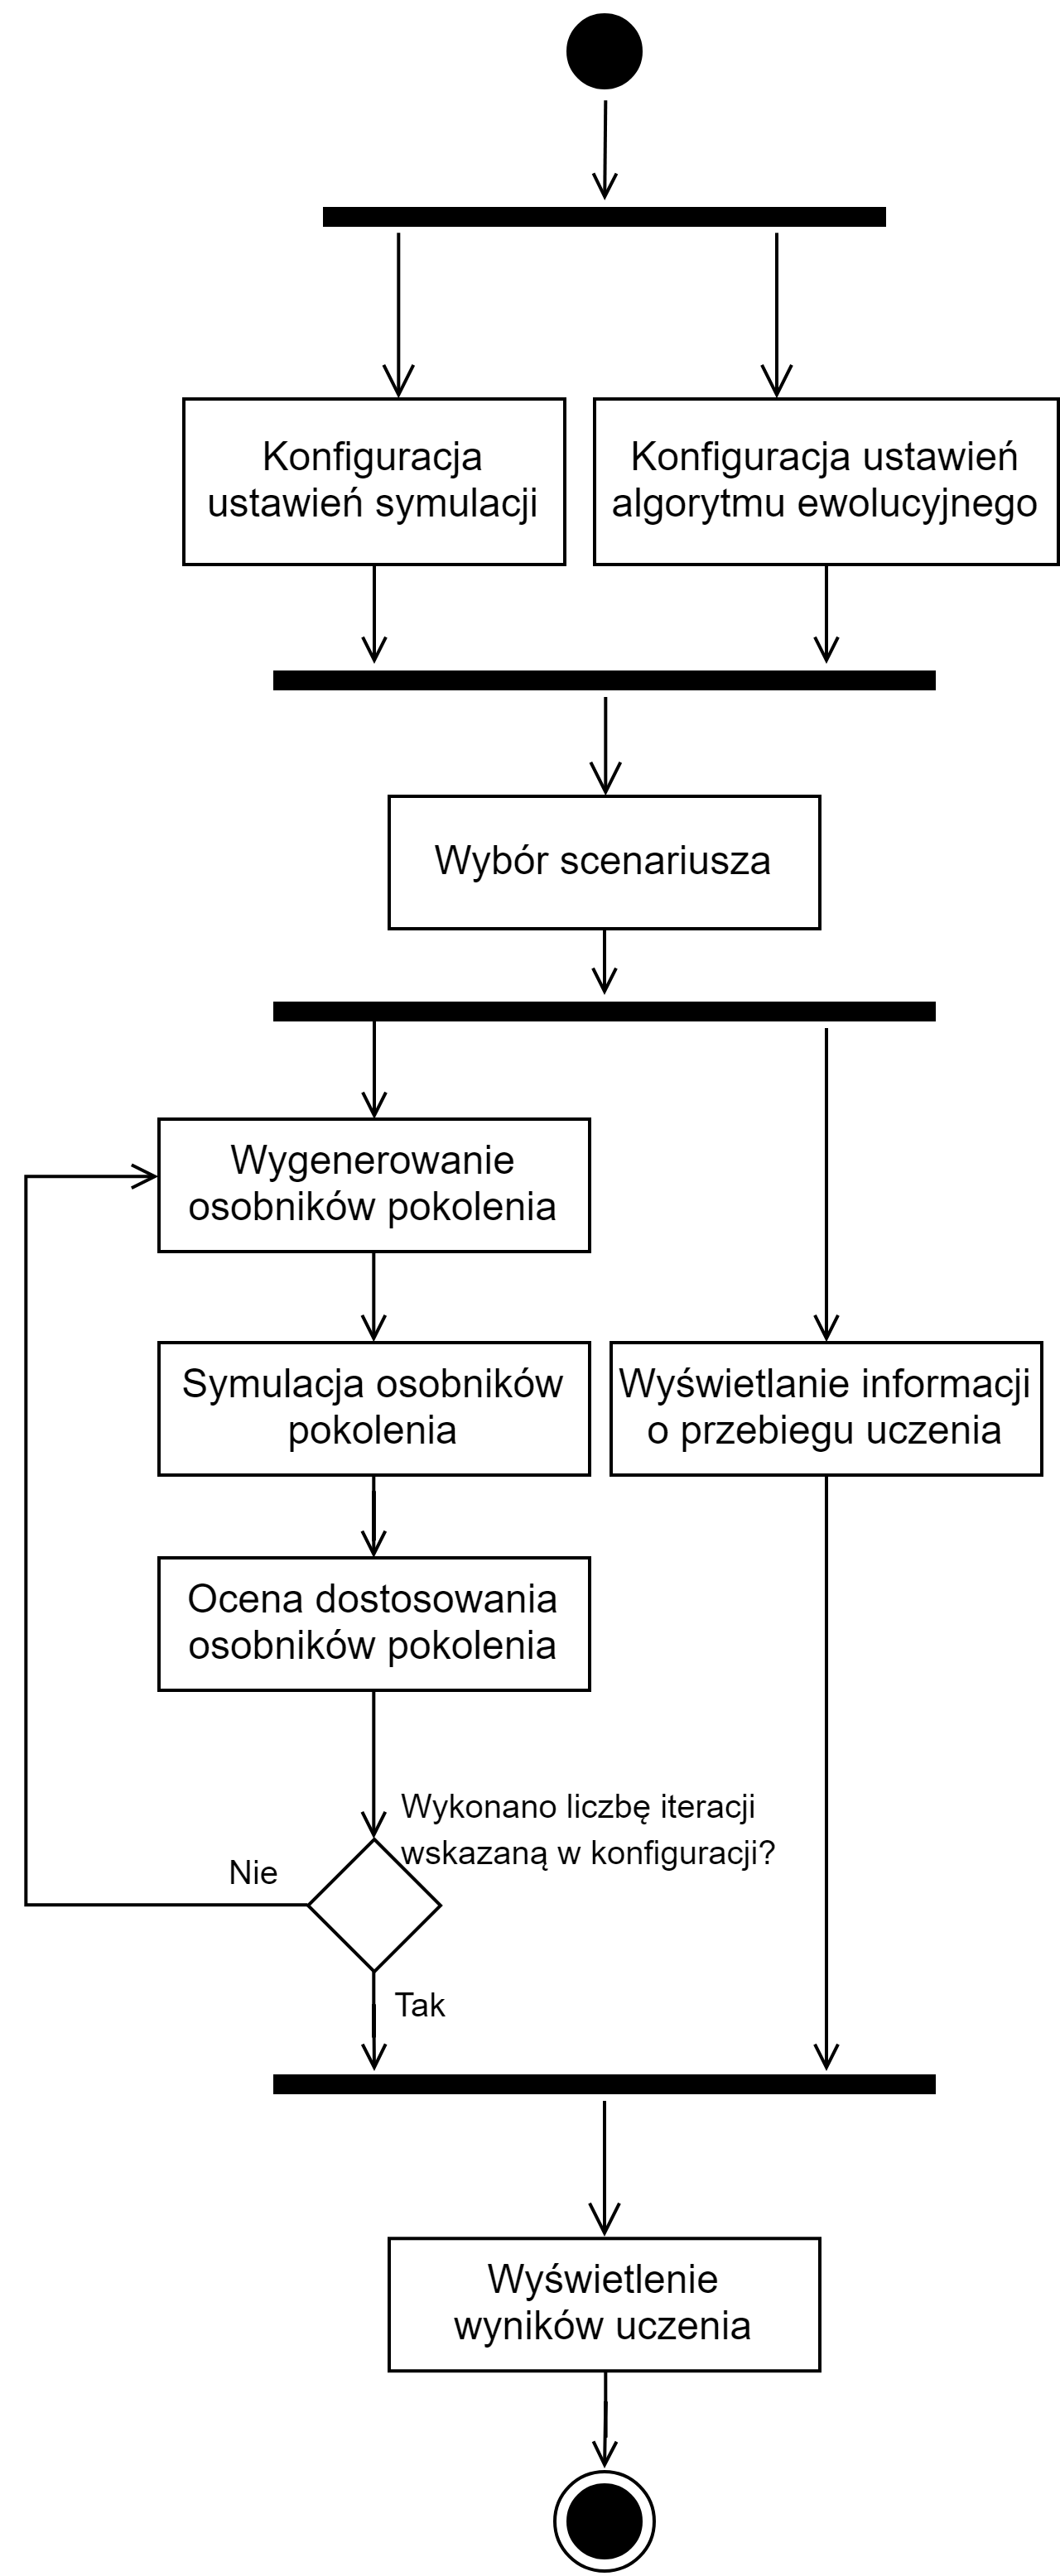
\includegraphics[height=0.9\textheight]{diagram_aktywnosci}
	\caption[Diagram aktywności aplikacji]{Diagram aktywności aplikacji}
	\label{fig:diagramaktywnosci}
\end{figure}

